\section{Evaluation}
\label{sec:Evaluation}
This section contains the evaluation and the graphical representation of the measurements.

\subsection{Slit Apertures}
\label{subsec:Slit}
The angle $\varphi$ was measured indirectly by measuring the distance from the slit aperture to the projection surface and the position of the maxima. All measured values are listed in appendix \ref{sec:Measurements} and the MATLAB code which calculates the angle using equation \ref{eq:angle} is listed in appendix \ref{sec:MATLAB_Angle_Calculation}.
\begin{figure}[H]
	\centering
	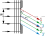
\includegraphics[scale=1]{slit}
	\caption{Slit Apertures}
	\label{fig:Slit}
\end{figure}
Figure \ref{fig:Slit} shows the indirectly measured angles $\varphi$ (see table \ref{tab:Slit_Measurements}) at several different orders $m$ and the according linear fit. The black dots were measured with the 40 $\mu$m slit aperture and the red squares were measured with the 100 $\mu$m slit aperture. To create the linear fit, equation \ref{eq:slit_maxima} was used for both slit apertures. The wavelength $\lambda$ was set to its according value (633 nm) and marked as constant.

The parameters of the linear fitted curve are listed in the following table:
\begin{table}[H]
	\centering
	\renewcommand{\arraystretch}{1.3}
	\begin{tabular}{r|c c}
		& \textbf{Slit 40 $\mu$m} & \textbf{Slit 100 $\mu$m} \\
		\hline\hline
		\textbf{Width} $w$ & $(39.41\pm0.10)$ $\mu$m & $(101.26\pm0.14)$ $\mu$m \\		
		\textbf{Wavelength} $\lambda$ & \multicolumn{2}{c}{633 nm (constant)}
	\end{tabular}
	\caption{Fit Parameters (Slit Apertures)}
	\label{tab:Slit}
\end{table}
\newpage
\subsection{Anti-Slit Apertures}
\label{subsec:Anti-Slit}
Once again the angle $\varphi$ was measured indirectly by measuring the distance from the anti-slit aperture to the projection surface and the position of the maxima. The measured values are listed in appendix \ref{sec:Measurements} and the MATLAB code used to calculate the angle is again listed in appendix \ref{sec:MATLAB_Angle_Calculation}.
\begin{figure}[H]
	\centering
	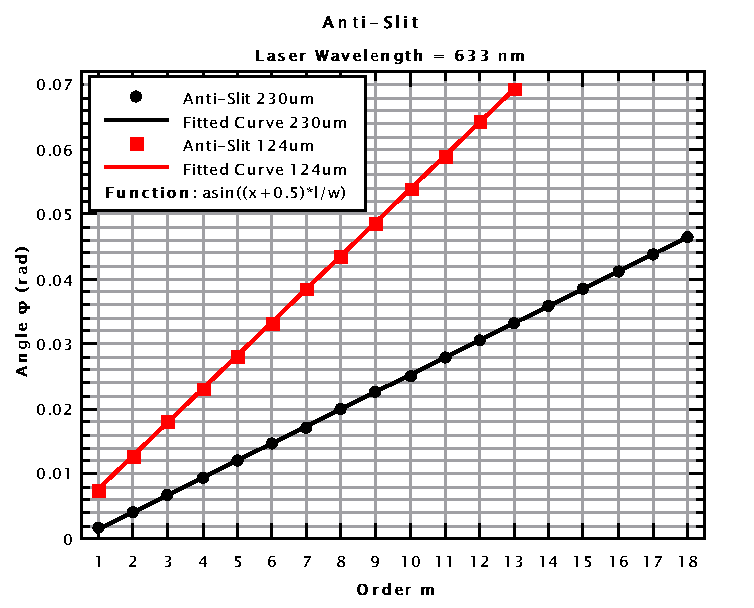
\includegraphics[scale=1]{anti-slit}
	\caption{Anti-Slit Apertures}
	\label{fig:Anti-Slit}
\end{figure}
Figure \ref{fig:Anti-Slit} shows the indirectly measured angles $\varphi$ (see table \ref{tab:Anti-Slit_Measurements}) at several different orders $m$ and the according linear fit. The black dots were measured with the 230 $\mu$m anti-slit aperture and the red squares were measured with the 124 $\mu$m anti-slit aperture. To create the linear fit, equation \ref{eq:slit_maxima} was used for both anti-slit apertures. The wavelength $\lambda$ was set to its according value (633 nm) and marked as constant.

The parameters of the linear fitted curve are listed in the following table:
\begin{table}[H]
	\centering
	\renewcommand{\arraystretch}{1.3}
	\begin{tabular}{r|c c}
		& \textbf{Anti-Slit 230 $\mu$m} & \textbf{Anti-Slit 124 $\mu$m} \\
		\hline\hline
		\textbf{Width} $w$ & $(239.10\pm0.34)$ $\mu$m & $(123.39\pm0.08)$ $\mu$m \\		
		\textbf{Wavelength} $\lambda$ & \multicolumn{2}{c}{633 nm (constant)}
	\end{tabular}
	\caption{Fit Parameters (Anti-Slit Apertures)}
	\label{tab:Anti-Slit}
\end{table}
\newpage
\subsection{Circular Apertures}
\label{subsec:Circular_Apertures}
The angle $\varphi$ was again measured indirectly by measuring the distance from the circular aperture to the projection surface. However, this time the positions of the minima were measured instead of the maxima. This is due to the lack of an easy equation to relate the maxima created by a circular aperture. The measured values are listed in appendix \ref{sec:Measurements} and the MATLAB code used to calculate the angle is listed in appendix \ref{sec:MATLAB_Angle_Calculation}.
\begin{figure}[H]
	\centering
	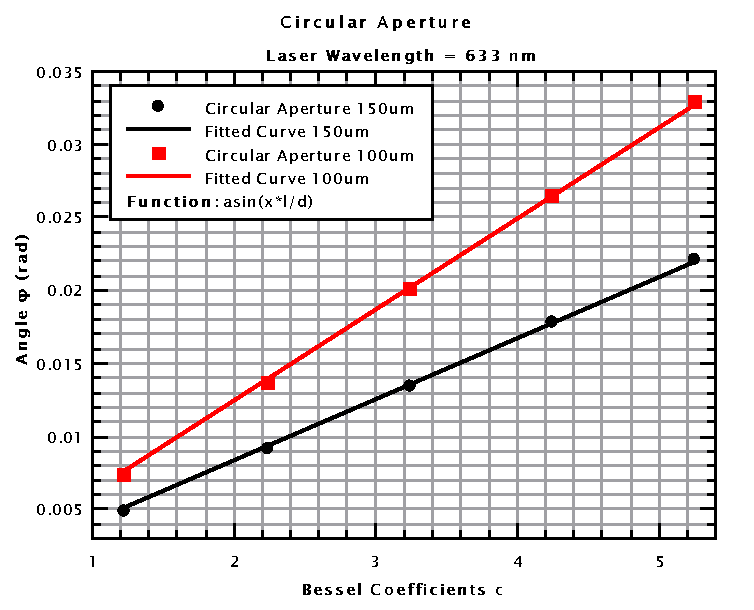
\includegraphics[scale=1]{circular_aperture}
	\caption{Circular Apertures}
	\label{fig:Circular_Apertures}
\end{figure}
Figure \ref{fig:Circular_Apertures} shows the indirectly measured angles $\varphi$ of the minima (see table \ref{tab:Circular_Apertures_Measurements}) at the first five Bessel coefficients $c_k$ (see equation \ref{eq:coeffs}) and the according linear fit. The black dots were measured with the 150 $\mu$m circular aperture and the red squares were measured with the 100 $\mu$m circular aperture. To create the linear fit, equation \ref{eq:circular_aperture} was used for both circular apertures. The wavelength $\lambda$ was set to its according value (633 nm) and marked as constant.

The parameters of the linear fitted curve are listed in the following table:
\begin{table}[H]
	\centering
	\renewcommand{\arraystretch}{1.3}
	\begin{tabular}{r|c c}
		& \textbf{Diameter 150 $\mu$m} & \textbf{Diameter 100 $\mu$m} \\
		\hline\hline
		\textbf{Diameter} $d$ & $(151.39\pm0.83)$ $\mu$m & $(101.62\pm0.55)$ $\mu$m \\		
		\textbf{Wavelength} $\lambda$ & \multicolumn{2}{c}{633 nm (constant)}
	\end{tabular}
	\caption{Fit Parameters (Circular Apertures)}
	\label{tab:Circular_Apertures}
\end{table}
\newpage
\subsection{Cross-Grid Apertures}
\label{subsec:Cross-Grid}
The angle $\varphi$ was measured indirectly by measuring the distance from the cross-grid aperture to the projection surface and the position of the maxima. All measured values are listed in appendix \ref{sec:Measurements} and the MATLAB code which calculates the angle using equation \ref{eq:angle} is listed in appendix \ref{sec:MATLAB_Angle_Calculation}.
\begin{figure}[H]
	\centering
	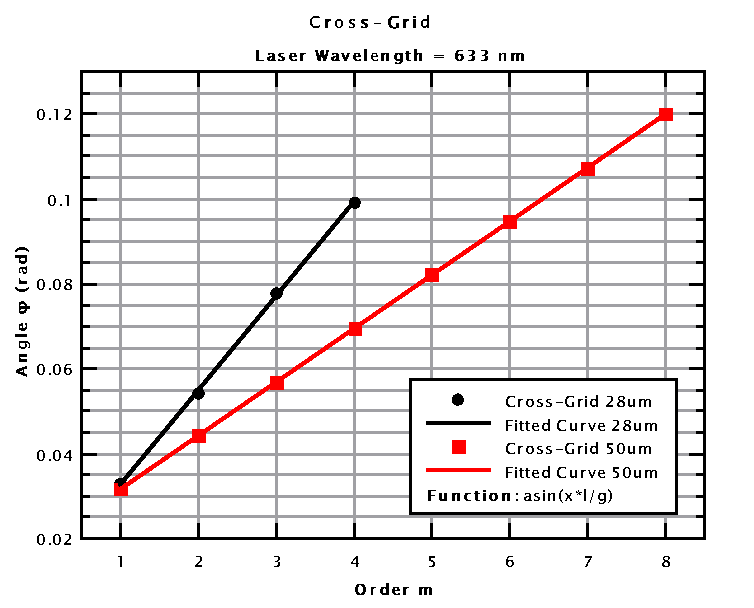
\includegraphics[scale=1]{cross-grid}
	\caption{Cross-Grid Apertures}
	\label{fig:Cross-Grid}
\end{figure}
Figure \ref{fig:Cross-Grid} shows the indirectly measured angles $\varphi$ (see table \ref{tab:Cross-Grid_Measurements}) at several orders $m$ and the according linear fit. The black dots were measured with a cross-grid that has a grid constant of 28 $\mu$m and the red squares were measured with a cross-grid that has a grid constant of 50 $\mu$m. To create the linear fit, equation \ref{eq:cross-grid} was used for both cross-grid apertures. The wavelength $\lambda$ was set to its according value (633 nm) and marked as constant.

The parameters of the linear fitted curve are listed in the following table:
\begin{table}[H]
	\centering
	\renewcommand{\arraystretch}{1.3}
	\begin{tabular}{r|c c}
		& \textbf{Cross-Grid 28 $\mu$m} & \textbf{Cross-Grid 50 $\mu$m} \\
		\hline\hline
		\textbf{Grid Constant} $g$ & $(28.53\pm0.44)$ $\mu$m & $(50.22\pm0.06)$ $\mu$m \\		
		\textbf{Wavelength} $\lambda$ & \multicolumn{2}{c}{633 nm (constant)}
	\end{tabular}
	\caption{Fit Parameters (Cross-Grid Apertures)}
	\label{tab:Cross-Grid}
\end{table}
